
% LaTeX Beamer file automatically generated from DocOnce
% https://github.com/hplgit/doconce

%-------------------- begin beamer-specific preamble ----------------------

\documentclass{beamer}

\usetheme{metropolis}
\usecolortheme{default}

% turn off the almost invisible, yet disturbing, navigation symbols:
\setbeamertemplate{navigation symbols}{}

% Exemples on customization:
%\usecolortheme[named=RawSienna]{structure}
%\usetheme[height=7mm]{Rochester}
%\setbeamerfont{frametitle}{family=\rmfamily,shape=\itshape}
%\setbeamertemplate{items}[ball]
%\setbeamertemplate{blocks}[rounded][shadow=true]
%\useoutertheme{infolines}
%
%\usefonttheme{}
%\useinntertheme{}
%
%\setbeameroption{show notes}
%\setbeameroption{show notes on second screen=right}

% fine for B/W printing:
%\usecolortheme{seahorse}

\usepackage{pgf}
\usepackage{graphicx}
\usepackage{epsfig}
\usepackage{relsize}

\usepackage{fancybox}  % make sure fancybox is loaded before fancyvrb

\usepackage{fancyvrb}
\usepackage{minted} % requires pygments and latex -shell-escape filename
%\usepackage{anslistings}
%\usepackage{listingsutf8}

\usepackage{amsmath,amssymb,bm}
%\usepackage[latin1]{inputenc}
\usepackage[T1]{fontenc}
\usepackage[utf8]{inputenc}
\usepackage{colortbl}
\usepackage[english]{babel}
\usepackage{tikz}
\usepackage{framed}
% Use some nice templates
\beamertemplatetransparentcovereddynamic

% --- begin table of contents based on sections ---
% Delete this, if you do not want the table of contents to pop up at
% the beginning of each section:
% (Only section headings can enter the table of contents in Beamer
% slides generated from DocOnce source, while subsections are used
% for the title in ordinary slides.)
\AtBeginSection[]
{
  \begin{frame}<beamer>[plain]
  \frametitle{}
  %\frametitle{Outline}
  \tableofcontents[currentsection]
  \end{frame}
}
% --- end table of contents based on sections ---

% If you wish to uncover everything in a step-wise fashion, uncomment
% the following command:

%\beamerdefaultoverlayspecification{<+->}

\newcommand{\shortinlinecomment}[3]{\note{\textbf{#1}: #2}}
\newcommand{\longinlinecomment}[3]{\shortinlinecomment{#1}{#2}{#3}}

\definecolor{linkcolor}{rgb}{0,0,0.4}
\hypersetup{
    colorlinks=true,
    linkcolor=linkcolor,
    urlcolor=linkcolor,
    pdfmenubar=true,
    pdftoolbar=true,
    bookmarksdepth=3
    }
\setlength{\parskip}{7pt}  % {1em}

\newenvironment{doconceexercise}{}{}
\newcounter{doconceexercisecounter}
\newenvironment{doconce:movie}{}{}
\newcounter{doconce:movie:counter}

\newcommand{\subex}[1]{\noindent\textbf{#1}}  % for subexercises: a), b), etc

\logo{{\tiny \copyright\ 2023, UP Mathématiques. ESPRIT}}

%-------------------- end beamer-specific preamble ----------------------

% Add user's preamble




% insert custom LaTeX commands...

\raggedbottom
\makeindex

%-------------------- end preamble ----------------------

\begin{document}

% matching end for #ifdef PREAMBLE

\newcommand{\exercisesection}[1]{\subsection*{#1}}



% ------------------- main content ----------------------



% ----------------- title -------------------------

\title{Introduction à Python (I)}

% ----------------- author(s) -------------------------

\author{UP Mathématiques\inst{1}}
\institute{École Supérieure PRivée d'Ingénierie et de Technologies.\inst{1}}
% ----------------- end author(s) -------------------------

\date{2 novembre 2023
% <optional titlepage figure>
\ \\ 
{\tiny \copyright\ 2023, UP Mathématiques. ESPRIT}
}

\begin{frame}[plain,fragile]
\titlepage
\end{frame}

\section{Objectifs généraux en premier}

\begin{frame}[plain,fragile]
\frametitle{Objectifs généraux en premier}


Une partie essentielle de ce cours est de vous permettre de faire de la science par des expériences numériques et de développer des projets qui vous permettent d'étudier des systèmes complexes. Le but est d'améliorer ce que nous appelons la pensée algorithmique.

\noindent\textbf{Algorithme}
Un ensemble fini d'instructions non ambiguës qui, étant donné un ensemble de conditions initiales, peuvent être effectuées dans une séquence prescrite pour atteindre un certain but.


\end{frame}

\section{Situation standard que nous rencontrons quotidiennement}

\begin{frame}[plain,fragile]
\frametitle{Situation standard que nous rencontrons quotidiennement}


La situation standard que nous rencontrons presque tous les séances de cours:

\begin{itemize}
\item Théorie + expérience + simulation est presque la norme dans la recherche et l'industrie.

\item Être capable de modéliser des systèmes complexes. Résoudre de vrais problèmes.

\item Accent la compréhension des principes fondamentaux et des lois dans les sciences.

\item Être capable de visualiser, présenter, discuter, interpréter et venir avec une analyse critique des résultats, et développer une attitude éthique saine pour son propre travail.

\item Améliorer le raisonnement sur la méthode scientifique.
\end{itemize}

\noindent
Une bonne présentation des résultats obtenus via de bons rapports scientifiques, aide à inclure tous les aspects ci-dessus.


\end{frame}

\section{Langage Python}

\begin{frame}[plain,fragile]
\frametitle{Langage Python}


\href{{http://www.python.org/}}{Python} est un langage de programmation moderne de haut niveau, orienté objet et d'usage général.

\textbf{Caractéristiques générales de Python} :

\begin{itemize}
\item Langage simple:
\begin{itemize}

  \item facile à lire et à apprendre avec une syntaxe minimaliste.

\end{itemize}

\noindent
\item Langage concis et expressif:
\begin{itemize}

  \item moins de lignes de code

  \item moins de bugs

  \item plus facile à maintenir.
\end{itemize}

\noindent
\end{itemize}

\noindent

\end{frame}

\begin{frame}[plain,fragile]
% No title on this slide

\textbf{Détails techniques} :

\begin{itemize}
\item Typé dynamiquement:
\begin{itemize}

  \item Pas besoin de définir le type des variables, les arguments ou le type des fonctions.

\end{itemize}

\noindent
\item La gestion automatique de la mémoire:
\begin{itemize}

  \item Aucune nécessité d'allouer explicitement et désallouer la mémoire pour les variables et les tableaux de données. Aucun bug de fuite de mémoire.

\end{itemize}

\noindent
\item Interprété:
\begin{itemize}

  \item Pas besoin de compiler le code. L'interpréteur Python lit et exécute le code python directement.
\end{itemize}

\noindent
\end{itemize}

\noindent
\end{frame}

\begin{frame}[plain,fragile]
% No title on this slide

\textbf{Avantages} :

\begin{itemize}
\item Le principal avantage est la facilité de programmation, qui minimise le temps nécessaire pour développer, déboguer et maintenir le code.

\item Langage bien conçu qui encourage les bonnes pratiques de programmation:
\begin{itemize}

  \item Modulaire et orientée objet, permet l'encapsulation  et la réutilisation de code. Il en résulte souvent un code plus transparent, plus facile à améliorer et sans bug.

  \item Documentation intégré avec le code.

\end{itemize}

\noindent
\item De nombreuses bibliothèques standards, et de nombreux packages add-on.
\end{itemize}

\noindent
\end{frame}

\begin{frame}[plain,fragile]
% No title on this slide

\vspace{6mm}

% inline figure
\centerline{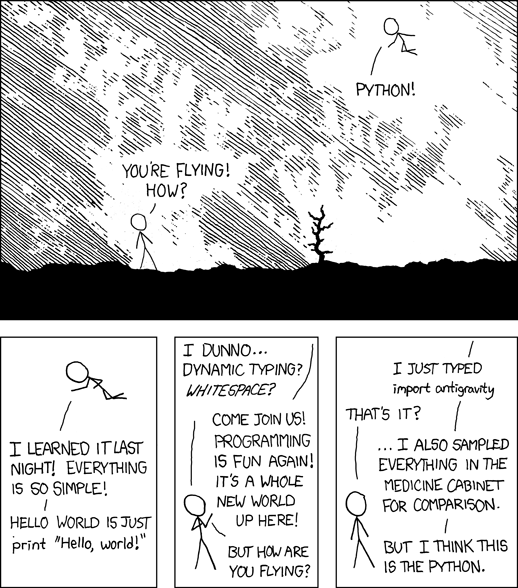
\includegraphics[width=0.6\linewidth]{imgs/python_easy.png}}

\vspace{6mm}
\end{frame}

\section{Installation d'un environnement Python scientifique}

\begin{frame}[plain,fragile]
\frametitle{Installation d'un environnement Python scientifique}




\noindent\textbf{Qu’est ce que Anaconda ?}
L’installation d’un environnement Python complet peut-être une vraie galère. Déjà, il faut télécharger Python et l’installer. Par la suite, télécharger un à un les packages dont on a besoin. Parfois, le nombre de ces librairies peut-être grand.

Par ailleurs, il faut s’assurer de la compatibilité entre les versions des différentes packages qu’on a à télécharger. Bref, ce n’est pas amusant.


\end{frame}

\begin{frame}[plain,fragile]
% No title on this slide

\href{{https://www.anaconda.com/download/}}{Anaconda} est  une distribution Python. A son installation, Anaconda installera Python ainsi qu'une multitude de packages (voir \href{{https://docs.anaconda.com/anaconda/packages/pkg-docs#python-3-6}}{liste de packages anaconda}).  Cela nous évite de nous ruer dans les problèmes d’incompatibilités entre les différents packages.

Finalement, Anaconda propose un outil de gestion de packages appelé \href{{https://conda.io/docs/}}{conda}. Ce dernier permettra de mettre à jour et installer facilement les librairies dont on aura besoin pour nos développements.
\end{frame}

\begin{frame}[plain,fragile]
% No title on this slide

\noindent\textbf{Préparer la formation: téléchargement d’Anaconda.}
Nous demandons à tous les étudiants de télécharger Anaconda. Pour cela, il faut télécharger un installeur à partir de \href{{https://www.anaconda.com/download/}}{\nolinkurl{https://www.anaconda.com/download/}}, correspondant à votre système d’exploitation (Windows, Mac OS X, Linux). Il faut choisir entre 32 bits ou 64 bits (pour la version \emph{Python 3}) selon que votre système d’exploitation est 32 bits ou 64 bits.
\end{frame}

\begin{frame}[plain,fragile]
% No title on this slide

\begin{figure}[!ht]  % 
  \centerline{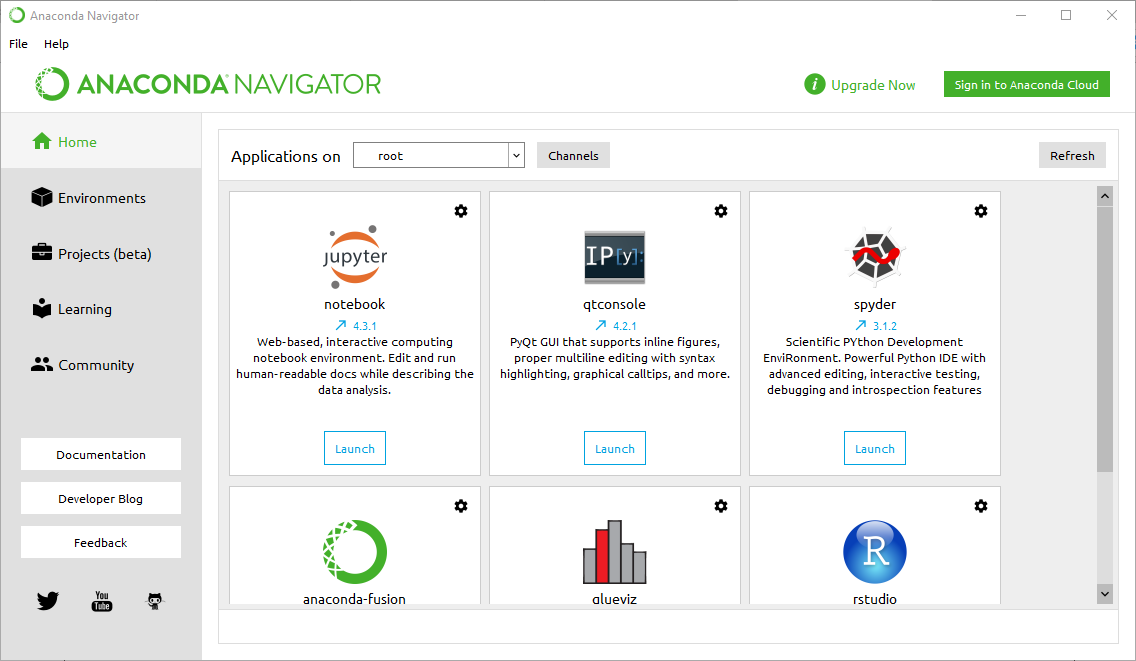
\includegraphics[width=0.7\linewidth]{imgs/AnacondaNavigator.png}}
  \caption{
  Interface graphique du navigateur Anaconda sur Windows
  }
\end{figure}
%\clearpage % flush figures
\end{frame}

\begin{frame}[plain,fragile]
% No title on this slide

\begin{block}{Note}
Anaconda installe plusieurs exécutables pour développer en Python dans le répertoire \emph{anaconda/bin}, sans toujours créer des raccourcis sur le bureau ou dans un menu. Nous nous occuperons au tout début de la formation de créer des raccourcis pour pouvoir lancer l'application web \emph{Jupyter notebook}. Vous pouvez lancer le notebook depuis le navigateur Anaconda.
\end{block}
\end{frame}

\section{Introduction: "Hello World!"}

\begin{frame}[plain,fragile]
\frametitle{Introduction: "Hello World!"}

C'est devenu une tradition que lorsque vous apprenez un nouveau langage de programmation, vous démarrez avec un programme permettant à l'ordinateur d'imprimer le message \emph{"Hello World!"}.

\begin{minted}[fontsize=\fontsize{9pt}{9pt},linenos=false,mathescape,baselinestretch=1.0,fontfamily=tt,xleftmargin=2mm]{python}
In [1]: print("Hello World!")
Hello World!
\end{minted}

Félicitation! tout à l'heure vous avez fait votre ordinateur saluer le monde en anglais! La fonction \texttt{print()} est utilisée pour imprimer l’instruction entre les parenthèses. De plus, l'utilisation de guillemets simples \Verb?print('Hello World!')? affichera le même résultat. Le délimiteur de début et de fin doit être le même.

\begin{minted}[fontsize=\fontsize{9pt}{9pt},linenos=false,mathescape,baselinestretch=1.0,fontfamily=tt,xleftmargin=2mm]{python}
In [2]: print('Hello World!')
Hello World!
\end{minted}


\end{frame}

\section{Commentaires}

\begin{frame}[plain,fragile]
\frametitle{Commentaires}


Au fur et à mesure que vos programmes deviennent plus grands et plus compliqués, ils deviennent plus difficiles à lire et à regarder un morceau de code et à comprendre ce qu'il fait ou pourquoi. Pour cette raison, il est conseillé d’ajouter des notes à vos programmes pour expliquer en langage naturel ce qu’il fait. Ces notes s'appellent des commentaires et commencent par le symbole \Verb!#!.

Voyez ce qui se passe lorsque nous ajoutons un commentaire au code précédent:

\begin{minted}[fontsize=\fontsize{9pt}{9pt},linenos=false,mathescape,baselinestretch=1.0,fontfamily=tt,xleftmargin=2mm]{python}
In [3]: print('Hello World!') # Ceci est mon premier commentaire
Hello World!
\end{minted}
Rien ne change dans la sortie? Oui, et c’est très normal, l’interprète Python ignore cette ligne et ne renvoie rien. La raison en est que les commentaires sont écrits pour les humains, pour comprendre leurs codes, et non pour les machines.


\end{frame}

\section{Nombres}

\begin{frame}[plain,fragile]
\frametitle{Nombres}


L'interpréteur Python agit comme une simple calculatrice: vous pouvez y taper une expression et l'interpréteur restituera la valeur. La syntaxe d'expression est simple: les opérateurs +, -, * et / fonctionnent comme dans la plupart des autres langages (par exemple, Pascal ou C); les parenthèses (\texttt{()}) peuvent être utilisées pour le regroupement. Par exemple:

\begin{minted}[fontsize=\fontsize{9pt}{9pt},linenos=false,mathescape,baselinestretch=1.0,fontfamily=tt,xleftmargin=2mm]{python}
In [4]: 5+3
Out[4]: 8
In [5]: 2 - 9      # les espaces sont optionnels
Out[5]: -7
In [6]: 7 + 3 * 4  #la hiérarchie des opérations mathématique
Out[6]: 19
In [7]: (7 + 3) * 4  # est-elle respectées?
Out[7]: 40
# en python3 la division retourne toujours un nombre en virgule flottante
In [8]: 20 / 3
Out[8]: 6.666666666666667
In [9]: 7 // 2      # une division entière
Out[9]: 3
\end{minted}


\end{frame}

\begin{frame}[plain,fragile]
% No title on this slide

On peut noter l’existence de l’opérateur \Verb!%! (appelé opérateur modulo). Cet opérateur fournit le reste de la division entière d’un nombre par un autre. Par exemple :

\begin{minted}[fontsize=\fontsize{9pt}{9pt},linenos=false,mathescape,baselinestretch=1.0,fontfamily=tt,xleftmargin=2mm]{python}
In [10]: 7 % 2       # donne le reste de la division
Out[10]: 1
In [11]: 6 % 2
Out[11]: 0
\end{minted}

Les exposants peuvent être calculés à l'aide de doubles astérisques \texttt{**}.

\begin{minted}[fontsize=\fontsize{9pt}{9pt},linenos=false,mathescape,baselinestretch=1.0,fontfamily=tt,xleftmargin=2mm]{python}
In [12]: 3**2
Out[12]: 9
\end{minted}

Les puissances de dix peuvent être calculées comme suit:

\begin{minted}[fontsize=\fontsize{9pt}{9pt},linenos=false,mathescape,baselinestretch=1.0,fontfamily=tt,xleftmargin=2mm]{python}
In [13]: 3 * 2e3   # vaut 3 * 2000
Out[13]: 6000.0
\end{minted}
\end{frame}

\section{Affectations (ou assignation)}

\begin{frame}[plain,fragile]
\frametitle{Affectations (ou assignation)}



Dans presque tous les programmes Python que vous allez écrire, vous aurez des variables. Les variables agissent comme des espaces réservés pour les données. Ils peuvent aider à court terme, ainsi qu’à la logique, les variables pouvant changer, d’où leur nom. C’est beaucoup plus facile en Python car aucune déclaration de variables n’est requise. Les noms de variable (ou tout autre objet Python tel que fonction, classe, module, etc.) commencent par une lettre majuscule ou minuscule (A-Z ou a-z). Ils sont sensibles à la casse (\texttt{VAR1} et \texttt{var1} sont deux variables distinctes). Depuis Python, vous pouvez utiliser n’importe quel caractère Unicode, il est préférable d’ignorer les caractères ASCII (donc pas de caractères accentués).

Si une variable est nécessaire, pensez à un nom et commencez à l'utiliser comme une variable, comme dans l'exemple ci-dessous:


\end{frame}

\begin{frame}[plain,fragile]
% No title on this slide

Pour calculer l'aire d'un rectangle par exemple: \texttt{largeur} x \texttt{hauteur}:
\begin{minted}[fontsize=\fontsize{9pt}{9pt},linenos=false,mathescape,baselinestretch=1.0,fontfamily=tt,xleftmargin=2mm]{python}
In [15]: largeur = 25
    ...: hauteur = 40
    ...: largeur    # essayer d'accéder à la valeur de la variable largeur
Out[15]: 25
\end{minted}


on peut également utiliser la fonction \texttt{print()} pour afficher la valeur de la variable \texttt{largeur}
\begin{minted}[fontsize=\fontsize{9pt}{9pt},linenos=false,mathescape,baselinestretch=1.0,fontfamily=tt,xleftmargin=2mm]{python}
In [16]: print(largeur)
25
\end{minted}
Le produit de ces deux variables donne l'aire du rectangle:
\begin{minted}[fontsize=\fontsize{9pt}{9pt},linenos=false,mathescape,baselinestretch=1.0,fontfamily=tt,xleftmargin=2mm]{python}
In [17]: largeur * hauteur  # donne l'aire du rectangle
Out[17]: 1000
\end{minted}
\end{frame}

\begin{frame}[plain,fragile]
% No title on this slide

\begin{block}{Note}
Notez ici que le signe égal (\texttt{=}) dans l'affectation ne doit pas être considéré comme \textbf{"est égal à"}. Il doit être \textbf{"lu"} ou interprété comme \textbf{"est définie par"}, ce qui signifie dans notre exemple:

\begin{quote}
La variable \texttt{largeur} est définie par la valeur 25 et la variable \texttt{hauteur} est définie par la valeur 40.
\end{quote}

\end{block}

\begin{block}{Avertissement}
Si une variable n'est pas \emph{définie} (assignée à une valeur), son utilisation vous donnera une erreur:

\begin{minted}[fontsize=\fontsize{9pt}{9pt},linenos=false,mathescape,baselinestretch=1.0,fontfamily=tt,xleftmargin=2mm]{python}
In [18]: aire     # essayer d'accéder à une variable non définie
-----------------------------------------------------------------------
NameError                            Traceback (most recent call last)
<ipython-input-18-1b03529c1ce5> in <module>()
----> 1 aire     # essayer d'accéder à une variable non définie

NameError: name 'aire' is not defined
\end{minted}
\end{block}
\end{frame}

\begin{frame}[plain,fragile]
\frametitle{Noms de variables réservés (keywords)}

Laissez-nous résoudre ce problème informatique (ou \textbf{bug} tout simplement)!. En d'autres termes, assignons la variable \texttt{aire} à sa valeur.

\begin{minted}[fontsize=\fontsize{9pt}{9pt},linenos=false,mathescape,baselinestretch=1.0,fontfamily=tt,xleftmargin=2mm]{python}
In [19]: aire = largeur * hauteur
    ...: aire  # et voila!
Out[19]: 1000
\end{minted}


Certains noms de variables ne sont pas disponibles, ils sont réservés à python lui-même. Les mots-clés suivants (que vous pouvez afficher dans l'interpréteur avec la commande \texttt{help("keywords")}) sont réservés et ne peuvent pas être utilisés pour définir vos propres identifiants (variables, noms de fonctions, classes, etc.).
\end{frame}

\begin{frame}[plain,fragile]
% No title on this slide

\begin{minted}[fontsize=\fontsize{9pt}{9pt},linenos=false,mathescape,baselinestretch=1.0,fontfamily=tt,xleftmargin=2mm]{python}
In [20]: help("keywords")

Here is a list of the Python keywords.  Enter any keyword to get more help.

False               def                 if                  raise
None                del                 import              return
True                elif                in                  try
and                 else                is                  while
as                  except              lambda              with
assert              finally             nonlocal            yield
break               for                 not
class               from                or
continue            global              pass

# par exemple pour éviter d'écraser le nom réservé lambda
In [22]: lambda_ = 630e-9
    ...: lambda_
Out[22]: 6.3e-07
\end{minted}
\end{frame}

\end{document}
